% !Mode:: "TeX:UTF-8"
%%% Local Variables:
%%% mode: latex
%%% TeX-master: t
%%% End:

\chapter{引言}
\label{chap:introduction}

\section{研究背景}

短波通信又称高频通信,是指使用频率范围在高频(HF)的无线电进行通信的方式\cite{董彬虹2007短波通信的现状及发展趋势}。短波通信主要利用天波电离层反射,所以无需中继站即可实现远距离通信,具有机动性强、设备成本低、对基础设施依赖小的优点,因此被广泛应用于广播、军事和抢险救灾等领域。

而同时,短波通信的缺陷也非常突出,因为受电离层变化和多径传播等因素的影响,短波通信的信道非常不稳定,导致其通信质量起伏较大,影响通信的稳定性。应对这一问题,军事中应用短波语音进行地空通信时,目前有一种解决方案:如图~\ref{fig:sys_struct}所示,在地面不同地点建立多个短波信号接收基站,接收来自空中飞机的短波语音。再将这多路信号汇总到一起,由人工选择一路质量最优的信号接入给地面指挥人员。人工选择需要的人工成本高,且稳定性和可靠性都不高,亟待使用算法代替人工。本文旨在通过对一系列算法及系统的研究,使用算法替代该方案中的人工选择步骤。

\begin{figure}
\centering
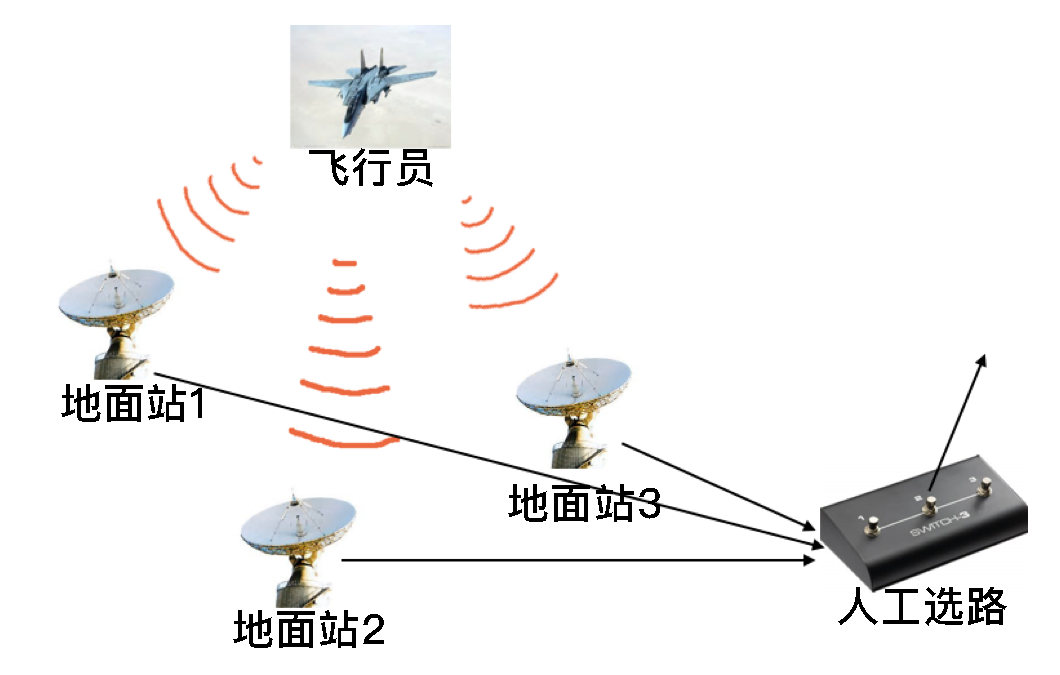
\includegraphics[width=0.8\textwidth]{sys_struct}
\caption{军事应用中的一种地空短波通信系统\label{fig:sys_struct}}
\end{figure}

\section{研究现状}


\subsection{背景模型及其在果蝇身体检测中的应用}


\section{研究目标和研究内容}

本文的主要目标在于研究果蝇活动台分割算法和果蝇轮廓提取算法,提升算法的鲁棒性,提升果蝇行为识别算法的应用范围。本文的研究内容主要包括:
\begin{enumerate}
\item 针对现有果蝇活动台提取算法的精确度较低的问题,本文引入了果蝇活动台的排列模式,通过将图像中的活动台和理想排列模式之间建立一一映射,去除果蝇活动台提取过程中的噪声。此外,对于不按照固定模式排列的果蝇活动台,引入自适应机制,减少该步骤中的人工干预;
\item 果蝇行为视频的实验环境和拍摄条件差异给果蝇轮廓提取带来很大的困难,针对此问题,本文提出一种果蝇轮廓提取算法,采用单高斯模型作为背景模型,通过亮度畸变区分果蝇翅膀和身体。初步建模后分离果蝇身体和活动台背景;然后在对活动台单独进建模的基础上,得到精确的背景模型用于轮廓提取。
\item 创建果蝇行为识别网站,对果蝇研究单位提供果蝇视频分析服务。
\end{enumerate}

\section{论文结构和内容概述}

本文剩余部分的结构如下所示:

第2章主要介绍果蝇活动台分割技术。介绍了如何通过调整HoughCircle算法参数,实现果蝇活动台的自适应提取和分割;然后,对基于特定排列的果蝇活动台,介绍通过坐标变换约束实现果蝇活动台位置校准的算法。最后,通过实验证明自适应步骤和排列信息能够提高果蝇活动台分割的性能。

第3章主要介绍果蝇轮廓提取和跟踪技术。首先,介绍一种基于单高斯模型的果蝇轮廓提取算法,然后在单高斯模型的基础上,提出一种针对果蝇活动台的背景模型,最后通过实验证明该模型对不同的视频具有较高的鲁棒性。

第4章主要采用第3章所提的果蝇身体提取算法,并在此基础上实现了果蝇行为识别的完整流程,通过实验给出了果蝇打架行为识别的准确率。实验证明,果蝇行为识别程序可以得到优于人工的识别结果。

第5章主要介绍了果蝇行为识别的网站,首先介绍了果蝇行为识别程序的功能模块、开发和部署环境,然后介绍了网站的基本功能和组成模块,以及其他研究者如何利用网站进行果蝇行为学研究。

第6章对本文工作进行总结,并对将来可能的研究方向进行展望。

